\phan{PHẦN I. PHẦN MỞ ĐẦU}
\label{phan:mo-dau}

\section*{1. Tính cấp thiết của đề tài}
\addcontentsline{toc}{section}{1. Tính cấp thiết của đề tài}

Thừa Thiên Huế là trung tâm văn hóa, lịch sử và du lịch đặc sắc hàng đầu của Việt Nam, sở hữu Quần thể Di tích Cố đô Huế được UNESCO vinh danh là Di sản Văn hóa Thế giới cùng hệ thống lăng tẩm triều Nguyễn, danh lam cổ tự và nền văn hóa ẩm thực cung đình lẫn dân gian trứ danh. Trong tiến trình xây dựng và phát triển tỉnh Thừa Thiên Huế trở thành thành phố trực thuộc Trung ương theo định hướng tại Nghị quyết số 54-NQ/TW của Bộ Chính trị, nhiệm vụ đẩy mạnh chuyển đổi số ngành du lịch và xây dựng hệ sinh thái đô thị thông minh đóng vai trò là đòn bẩy phát triển kinh tế xã hội trọng điểm. Cùng với sự bùng nổ của các mô hình ngôn ngữ lớn (Large Language Models -- LLM) và trí tuệ nhân tạo tạo sinh, hành vi của du khách hiện đại đã có sự chuyển biến căn bản: người dùng ngày càng có nhu cầu tương tác với các trợ lý ảo đàm thoại thông minh có khả năng thấu hiểu ngữ cảnh tự nhiên, tư vấn lịch trình cá nhân hóa, gợi ý địa điểm ẩm thực địa phương chuẩn xác và tối ưu hóa tuyến đường theo thời gian thực thay vì tra cứu thủ công qua các danh bạ tĩnh truyền thống.

Tuy nhiên, trong thực tiễn công tác quản lý và xúc tiến du lịch tại địa phương, ngành du lịch Thừa Thiên Huế đang đứng trước bài toán chiến lược mang tính sống còn về việc kéo dài thời gian lưu trú và gia tăng mức chi tiêu của du khách. Vấn đề cấp bách này đã được lãnh đạo Thành phố Huế đặc biệt nhấn mạnh trong chuyến khảo sát thực địa và chỉ đạo điều hành vào tháng 9 năm 2026, được cơ quan báo chí phản ánh rộng rãi, tiêu biểu như bài viết trên Báo Thanh Niên~\cite{thanhnien2026tourism} được ghi nhận tại Hình~\ref{fig:thanhnien-tourism}.

\begin{figure}[htbp]
    \centering
    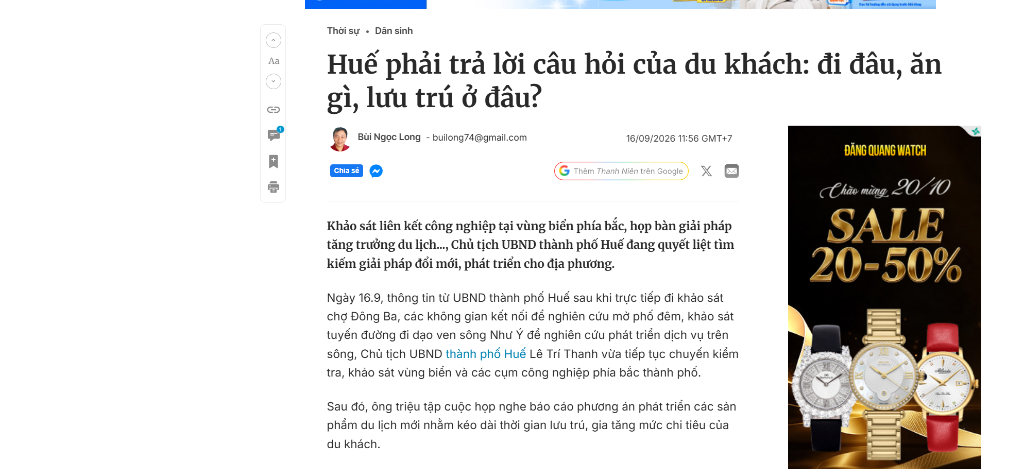
\includegraphics[width=0.88\textwidth]{img/thanhnien_hue_tourism_problem.png}
    \caption{Bài báo phản ánh chỉ đạo của lãnh đạo thành phố Huế về yêu cầu giải quyết ba câu hỏi cốt lõi của du khách: Đi đâu, ăn gì, lưu trú ở đâu trên Báo Thanh Niên~\cite{thanhnien2026tourism}.}
    \label{fig:thanhnien-tourism}
\end{figure}

Từ nội dung chỉ đạo thực tế được phản ánh trên Hình~\ref{fig:thanhnien-tourism}, lãnh đạo chính quyền Thành phố Huế sau các chuyến kiểm tra thực địa tại chợ Đông Ba, các không gian kết nối phát triển phố đêm và tuyến đường đi dạo ven sông Như Ý đã triệu tập cuộc họp chuyên đề nhằm tìm kiếm các giải pháp đột phá. Thông điệp cốt lõi được đặt ra cho toàn ngành du lịch Cố đô là: \textit{Huế phải trả lời một cách thỏa đáng, tức thời và thuyết phục ba câu hỏi căn bản của du khách: Đi đâu? Ăn gì? Lưu trú ở đâu?}. Nếu không giải quyết thấu đáo chuỗi nhu cầu liên hoàn này, du khách sẽ chỉ đến Huế theo hình thức tham quan chớp nhoáng ban ngày rồi di chuyển sang các địa phương lân cận, khiến ngành du lịch địa phương bỏ lỡ nguồn doanh thu dịch vụ và kinh tế đêm to lớn.

Nhằm hiện thực hóa mục tiêu chuyển đổi số phục vụ người dân và du khách, tỉnh Thừa Thiên Huế đã tiên phong xây dựng nền tảng đô thị thông minh Hue-S~\cite{hues2024}, tích hợp phân hệ thông tin du lịch và dịch vụ công dân số. Dù đạt được nhiều thành tựu quan trọng về mặt chính quyền điện tử, khi đi sâu vào phân hệ hỗ trợ du lịch tương tác, ứng dụng Hue-S hiện tại vẫn bộc lộ những hạn chế kỹ thuật đáng kể, được minh họa trực quan thông qua hai giao diện thực tế tại Hình~\ref{fig:hues-analysis}.

\begin{figure}[htbp]
    \centering
    \begin{subfigure}[b]{0.47\textwidth}
        \centering
        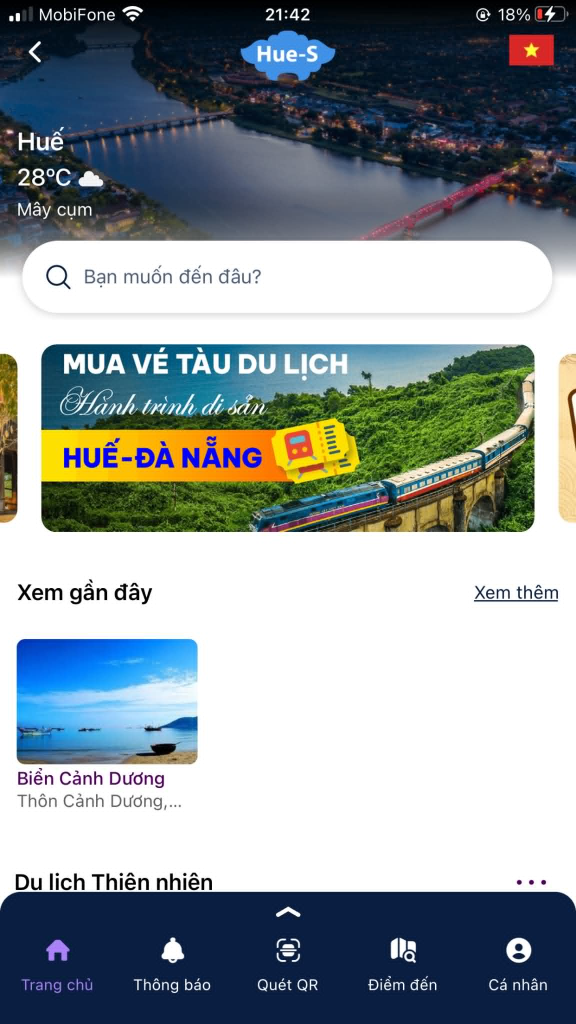
\includegraphics[width=\textwidth]{img/hues_smart_city_app_home.png}
        \caption{Giao diện chính phân hệ du lịch trên Hue-S}
        \label{subfig:hues-home}
    \end{subfigure}
    \hfill
    \begin{subfigure}[b]{0.47\textwidth}
        \centering
        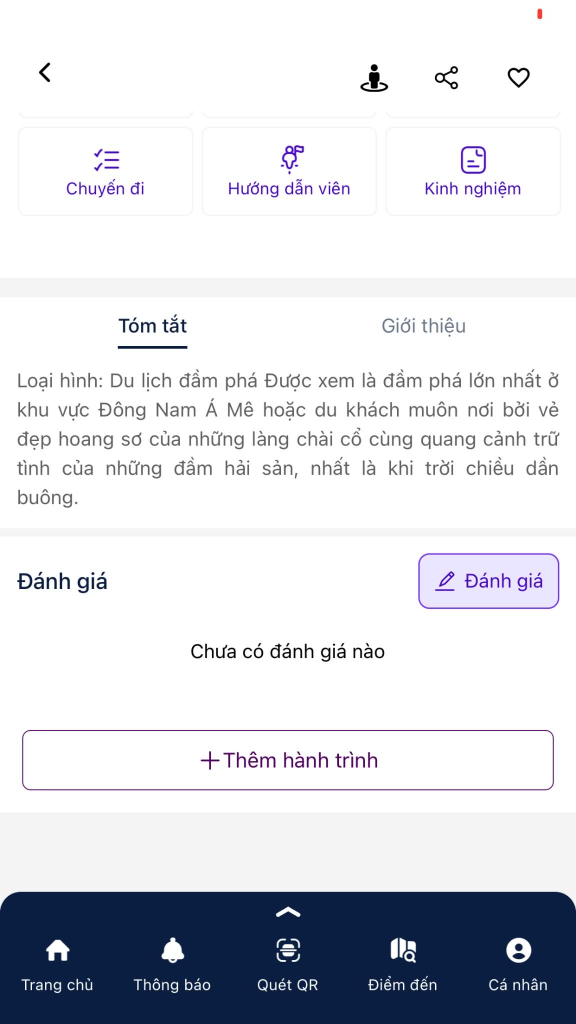
\includegraphics[width=\textwidth]{img/hues_app_limitation_review.png}
        \caption{Chi tiết điểm đến bộc lộ hạn chế đánh giá và lập lịch}
        \label{subfig:hues-detail}
    \end{subfigure}
    \caption{Thực trạng giao diện phân hệ du lịch trên nền tảng đô thị thông minh Hue-S cho thấy sự thiếu vắng dữ liệu đánh giá thực tế và công cụ lập lịch trình tự động~\cite{hues2024}.}
    \label{fig:hues-analysis}
\end{figure}

Quan sát giao diện thực tế tại Hình~\ref{subfig:hues-home}, phân hệ du lịch của Hue-S hiện tại hoạt động theo mô hình cổng thông tin điện tử một chiều: cung cấp thanh tìm kiếm từ khóa cơ bản, thông tin thời tiết, quảng bá dịch vụ vé tàu di sản tuyến Huế -- Đà Nẵng và danh mục các điểm đến phân theo nhóm thiên nhiên hoặc di tích. Tuy nhiên, khi người dùng truy cập sâu vào chi tiết của một địa danh du lịch (như điểm đến du lịch đầm phá Tam Giang -- Cầu Hai trên Hình~\ref{subfig:hues-detail}), hệ thống bộc lộ hai rào cản trải nghiệm hết sức rõ rệt. Thứ nhất, tại mục \textit{Đánh giá}, hệ thống thông báo trạng thái \textit{``Chưa có đánh giá nào''}. Điều này phản ánh thực trạng thiếu hụt trầm trọng cơ sở dữ liệu phản hồi thực tế từ cộng đồng du khách (Cold-start Review Gap), thiếu vắng các thuật toán phân tích cảm xúc (Sentiment Analysis) và hoàn toàn không có khả năng khai phá thị hiếu ẩm thực hay các món ăn đặc sản được yêu thích tại địa phương. Thứ hai, nút bấm chức năng \textit{Thêm hành trình} chỉ đóng vai trò như một danh sách đánh dấu (bookmark) thủ công thụ động. Người dùng phải tự tìm kiếm địa điểm, tự căn chỉnh cự ly và tự ước lượng thời gian di chuyển mà không nhận được bất kỳ sự hỗ trợ nào từ thuật toán tối ưu hóa tuyến đường có nhận thức không gian (Spatial Routing Engine).

Để giải quyết khoảng trống giữa kỳ vọng của du khách và năng lực của các ứng dụng du lịch hiện hành, xu hướng ứng dụng trí tuệ nhân tạo tạo sinh mở ra tiềm năng lớn. Dẫu vậy, việc áp dụng trực tiếp các mô hình ngôn ngữ lớn thương mại hoặc các hệ thống Tăng cường Tạo sinh Truy xuất truyền thống (Naive RAG) vào miền du lịch địa phương tại Huế đang vấp phải ba thách thức kỹ thuật cốt lõi:

Thách thức thứ nhất xuất phát từ hiện tượng ảo giác thực thể địa phương (Local Entity Hallucination). Do dữ liệu tiền huấn luyện của các mô hình LLM chủ yếu dựa trên ngữ liệu tổng quát toàn cầu, mô hình thường xuyên tự bịa đặt tên các quán ăn, nhà hàng nghe có vẻ giống tiếng Việt nhưng hoàn toàn không tồn tại trong thực tế tại Huế, hoặc gán ghép sai lệch giữa đặc sản các vùng miền. Tình trạng này làm suy giảm nghiêm trọng độ tin cậy của hệ thống tư vấn và có thể gây phương hại trực tiếp đến trải nghiệm thực địa của du khách.

Thách thức thứ hai là khiếm khuyết thiếu nhận thức không gian (Space-agnostic limitation). Bản chất của cơ chế tìm kiếm tương đồng véc-tơ trong Naive RAG thuần túy dựa trên sự tương đồng ngữ nghĩa văn bản mà hoàn toàn không nắm bắt được tọa độ địa lý, địa hình tự nhiên và cự ly di chuyển thực tế. Tại một đô thị có địa hình đặc thù bị chia cắt bởi dòng sông Hương như thành phố Huế, sự thiếu hụt này dẫn đến những lịch trình hết sức phi lý: hệ thống liên tục gợi ý du khách di chuyển ziczac qua lại giữa bờ Bắc (khu vực di sản Kinh thành) và bờ Nam (khu vực phố mới và các lăng tẩm), hoặc gợi ý các quán ăn cách xa điểm tham quan hàng chục kilômét trong khi du khách đang có nhu cầu đi bộ lân cận.

Thách thức thứ ba nằm ở sự chia cắt giữa dữ liệu đánh giá thực tế và cấu trúc biểu diễn tri thức. Thông tin đăng ký kinh doanh chính thống của các nhà hàng, quán ăn thường chỉ cung cấp danh mục chung chung, thiếu sự kiểm chứng về chất lượng thực tế. Trong khi đó, hàng chục ngàn bài nhận xét của du khách trên các nền tảng trực tuyến như TripAdvisor lại chứa đựng nguồn tri thức ngầm vô cùng phong phú về các món ăn đặc sản được yêu thích nhất tại từng địa điểm nhưng chưa được khai phá và liên kết có cấu trúc vào cơ sở tri thức.

Xuất phát từ những đòi hỏi thực tiễn của chính quyền thành phố Huế và khoảng trống học thuật nêu trên, đề tài \textbf{\tendetai} được đề xuất nhằm nghiên cứu và xây dựng một khung giải pháp toàn diện: tích hợp Đồ thị Tri thức Không gian (Spatial Knowledge Graph) với mô hình ngôn ngữ lớn cục bộ thông qua kiến trúc tác tử đa luồng (Agentic RAG). Giải pháp này hướng tới mục tiêu triệt tiêu ảo giác địa danh, tối ưu hóa cung đường di chuyển theo cụm địa lý và khai phá khẩu vị ẩm thực du khách, qua đó trả lời một cách tự động và chuẩn xác ba câu hỏi cốt lõi: Đi đâu, ăn gì và lưu trú ở đâu phục vụ đắc lực cho công tác quảng bá du lịch Cố đô Huế.

\section*{2. Mục tiêu nghiên cứu}
\addcontentsline{toc}{section}{2. Mục tiêu nghiên cứu}

Mục tiêu tổng quát của khóa luận là thiết kế, hiện thực hóa và đánh giá định lượng một hệ thống hỏi đáp và gợi ý lịch trình du lịch thông minh mang tên Spatial GraphRAG, kết hợp cấu trúc Đồ thị Tri thức Không gian, dữ liệu phản hồi thực tế của du khách và khung tác tử điều phối đa luồng trên nền tảng mô hình ngôn ngữ lớn cục bộ, nhằm cung cấp các đề xuất du lịch chuẩn xác về mặt thực thể và tối ưu về mặt cự ly địa lý tại thành phố Huế.

Để đạt được mục tiêu tổng quát, nghiên cứu xác lập bốn mục tiêu cụ thể.

Mục tiêu cụ thể thứ nhất là xây dựng Đồ thị Tri thức Không gian du lịch hoàn chỉnh cho Huế và các tỉnh thành trọng điểm với quy mô hơn 9.500 nút thực thể và hơn 90.000 cạnh quan hệ ngữ nghĩa, tích hợp thuộc tính tọa độ GPS chuẩn WGS84 và bán kính lân cận thực tế theo công thức khoảng cách mặt cầu Haversine.

Mục tiêu cụ thể thứ hai là xây dựng bộ từ điển ẩm thực Việt Nam gồm 570 món ăn (trong đó có hơn 60 món đặc sản Huế) và thiết lập giải thuật khai phá tri thức ngầm từ tập ngữ liệu 44.355 bài đánh giá du khách thực tế tại Huế trên nền tảng TripAdvisor để liên kết tự động quan hệ phục vụ món ăn vào đồ thị với độ tin cậy thống kê cao.

Mục tiêu cụ thể thứ ba là thiết kế khung điều phối Agentic RAG trên LangGraph tích hợp bộ chấm điểm tin cậy (Confidence Grading) và cơ chế phân luồng dự phòng tìm kiếm Internet, vận hành hoàn toàn trên mô hình ngôn ngữ mã nguồn mở cục bộ Qwen2.5-3B nhằm bảo đảm quyền riêng tư của du khách và triệt tiêu toàn bộ chi phí bản quyền API vận hành.

Mục tiêu cụ thể thứ tư là hiện thực hóa giải thuật lập lịch trình phân cụm địa lý (Spatial Itinerary Planner), phát triển giao diện Web tương tác bản đồ số trực quan và đóng gói Cổng API RESTful chuẩn mở sẵn sàng tích hợp với nền tảng công dân số Hue-S.

\section*{3. Câu hỏi nghiên cứu và Giả thuyết khoa học}
\addcontentsline{toc}{section}{3. Câu hỏi nghiên cứu và Giả thuyết khoa học}

Tiến trình nghiên cứu được định hướng bởi bốn câu hỏi nghiên cứu cốt lõi:

Câu hỏi nghiên cứu RQ1: Làm thế nào để mô hình hóa mối quan hệ không gian giữa các điểm tham quan, nhà hàng ẩm thực và cơ sở lưu trú thành một Đồ thị Tri thức Không gian có khả năng truy vấn hiệu quả theo bán kính địa lý thực tế?

Câu hỏi nghiên cứu RQ2: Cơ chế trích xuất thực đơn ngầm từ hàng chục ngàn bài đánh giá văn bản phi cấu trúc của du khách có thể nâng cao độ chính xác và độ phong phú của việc gợi ý món ăn đặc sản so với dữ liệu phân loại tĩnh truyền thống ở mức độ nào?

Câu hỏi nghiên cứu RQ3: Việc tích hợp Đồ thị Tri thức Không gian vào quy trình RAG (Spatial GraphRAG) có thể triệt tiêu hiện tượng ảo giác thực thể và giảm thiểu tỷ lệ vi phạm cự ly di chuyển so với Naive RAG và Zero-shot LLM ra sao?

Câu hỏi nghiên cứu RQ4: Khung tác tử LangGraph kết hợp mô hình ngôn ngữ cục bộ quy mô nhỏ (Qwen2.5-3B) có đáp ứng được yêu cầu về thời gian phản hồi thời gian thực và độ chính xác tổng thể khi vận hành trên hạ tầng máy trạm tiêu chuẩn hay không?

Tương ứng với các câu hỏi nghiên cứu nêu trên, khóa luận xác lập bốn giả thuyết khoa học:

Giả thuyết khoa học $H_1$: Ràng buộc topo không gian (cạnh liên kết lân cận trong bán kính mặt cầu $d \le 1,5\text{ km}$) sẽ triệt tiêu hoàn toàn các lộ trình ziczac nhảy bờ sông Hương vô lý, giảm cự ly di chuyển trung bình ít nhất 50\% so với hệ thống Naive RAG truyền thống.

Giả thuyết khoa học $H_2$: Khai phá thực đơn ngầm từ tập ngữ liệu nhận xét du khách cho phép mở rộng độ phủ món ăn đặc sản lên trên 90\%, vượt trội so với danh mục ẩm thực phân loại tĩnh.

Giả thuyết khoa học $H_3$: Mô hình Spatial GraphRAG đạt tỷ lệ bảo chứng thực thể (Grounding Rate) 100\% và tỷ lệ ảo giác địa danh 0\% trên toàn bộ các truy vấn kiểm thử thuộc phạm vi đồ thị tri thức.

Giả thuyết khoa học $H_4$: Quy trình phân cụm lịch trình theo không gian kết hợp bộ lập lịch trình thông minh bảo đảm thời gian sinh kết quả dưới 4 giây trên GPU cá nhân, hoàn toàn đủ điều kiện cung cấp dịch vụ trực tuyến ổn định trong điều kiện thực tế.

\section*{4. Đối tượng và Phạm vi nghiên cứu}
\addcontentsline{toc}{section}{4. Đối tượng và Phạm vi nghiên cứu}

Đối tượng nghiên cứu của khóa luận là các phương pháp biểu diễn tri thức không gian (Spatial Knowledge Representation), kỹ thuật Tăng cường Tạo sinh Truy xuất dựa trên đồ thị (GraphRAG), khung điều phối tác tử hội thoại thông minh (Agentic Workflows) và các giải thuật tối ưu hóa lịch trình du lịch dựa trên địa lý. Về mặt dữ liệu, đối tượng nghiên cứu bao gồm 9.525 thực thể điểm du lịch, ẩm thực, lưu trú và 44.355 bản ghi đánh giá du khách thực tế tại Huế thu thập từ TripAdvisor, kết hợp dữ liệu tọa độ hình học từ OpenStreetMap và Google Maps.

Về phạm vi nghiên cứu, không gian địa lý trọng tâm của đề tài được định vị tại thành phố Huế và các vùng phụ cận thuộc tỉnh Thừa Thiên Huế (khu vực Kinh thành, cụm lăng tẩm phía Nam, đầm Chuồn, đầm phá Tam Giang, làng cổ Phước Tích, cầu ngói Thanh Toàn). Các thực thể tại các tỉnh thành du lịch lân cận (Đà Nẵng, Quảng Nam) đóng vai trò làm giàu ngữ cảnh đồ thị liên kết vùng. Về mặt công nghệ, nghiên cứu tập trung vào mô hình ngôn ngữ cục bộ Qwen2.5-3B-Instruct vận hành qua môi trường Ollama trên GPU NVIDIA GeForce RTX 3050 (4GB VRAM), bảo đảm tính khả thi triển khai và vận hành tự chủ hoàn toàn tại các cơ quan, đơn vị địa phương.

\section*{5. Ý nghĩa khoa học và Thực tiễn}
\addcontentsline{toc}{section}{5. Ý nghĩa khoa học và Thực tiễn}

Về mặt khoa học, khóa luận đóng góp một khung phương pháp luận mới kết hợp giữa tính toán không gian (Spatial Computing) và GraphRAG. Nghiên cứu làm rõ cơ chế tích hợp khoảng cách mặt cầu Haversine vào cấu trúc đồ thị tri thức, đồng thời đề xuất giải pháp dung hợp giữa tri thức có cấu trúc của đồ thị và tri thức phi cấu trúc từ nhận xét du khách để định hướng quá trình suy luận của LLM mà không cần tái huấn luyện mô hình nền tảng.

Về mặt thực tiễn, sản phẩm của đề tài mang lại giá trị ứng dụng trực tiếp cho ngành du lịch Thừa Thiên Huế. Hệ thống không chỉ cung cấp giải pháp trợ lý ảo thông minh giúp du khách tự lập kế hoạch du lịch tiết kiệm thời gian và chi phí, mà còn sẵn sàng kết nối API vào nền tảng số Hue-S, hỗ trợ chính quyền địa phương giải quyết bài toán: Đi đâu, ăn gì, lưu trú ở đâu, điều tiết dòng khách du lịch hợp lý giữa các cụm di sản, góp phần bảo tồn di tích và thúc đẩy kinh tế đêm bền vững.

\section*{6. Cấu trúc của khóa luận}
\addcontentsline{toc}{section}{6. Cấu trúc của khóa luận}

Khóa luận được kết cấu thành năm phần theo đúng quy định tại Văn bản số 1967/HD-ĐHH của Đại học Huế:

Phần I trình bày phần mở đầu với tính cấp thiết của đề tài gắn liền với chỉ đạo thực tiễn của lãnh đạo thành phố Huế và hiện trạng ứng dụng Hue-S, mục tiêu nghiên cứu, câu hỏi nghiên cứu, đối tượng và phạm vi đề tài.

Phần II tổng quan cơ sở lý thuyết nền tảng về Đồ thị Tri thức Không gian, tiến trình phát triển từ Naive RAG sang GraphRAG và Agentic RAG, mô hình không gian véc-tơ, bài toán thiết kế chuyến đi du lịch TTDP, và các công trình liên quan.

Phần III làm rõ đối tượng, nguồn dữ liệu 44.355 đánh giá TripAdvisor tại Huế, quy trình làm sạch dữ liệu và phương pháp luận thiết kế hệ thống.

Phần IV là nội dung và kết quả nghiên cứu, bao gồm Chương 1 trình bày chi tiết kiến trúc 4 tầng của Spatial GraphRAG cùng giải thuật khai phá thực đơn ngầm, và Chương 2 trình bày thuật toán lập lịch trình không gian, kết quả thực nghiệm đối sánh định lượng trên bộ benchmark 12 kịch bản và kiến trúc cổng tích hợp Hue-S.

Phần V tổng kết các đóng góp chính của đề tài, phân tích trung thực các hạn chế hiện tại và định hướng phát triển trong tương lai.
